\begin{question}
\noindent A science museum displays two similar spherical model planets, used to represent a planet and its larger counterpart in an exhibit about scale in the solar system. The two spheres are mathematically similar, with radii in the ratio $3:5$.

\begin{center}
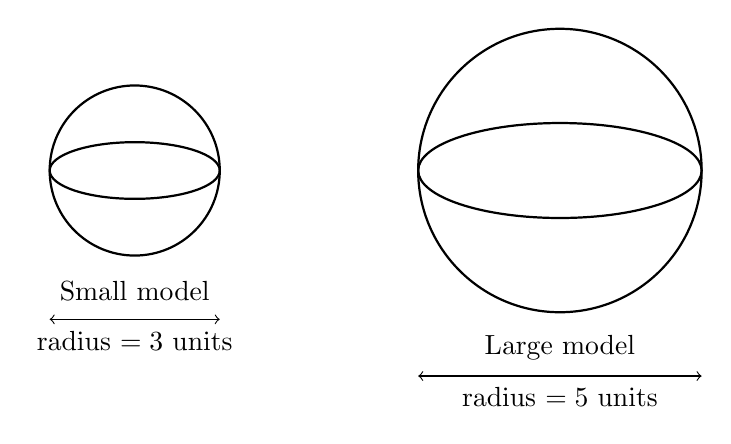
\begin{tikzpicture}[scale=0.9]
    % Smaller sphere
    \draw[thick] (0,0) circle (1.2cm);
    \draw[thick] (0,0) ellipse (1.2cm and 0.4cm);
    \node at (0,-1.7) {Small model};
    \draw[<->] (-1.2,-2.1) -- (1.2,-2.1);
    \node at (0,-2.4) {radius $= 3$ units};

    % Larger sphere
    \draw[thick] (6,0) circle (2cm);
    \draw[thick] (6,0) ellipse (2cm and 0.67cm);
    \node at (6,-2.5) {Large model};
    \draw[<->] (4,-2.9) -- (8,-2.9);
    \node at (6,-3.2) {radius $= 5$ units};
\end{tikzpicture}
\end{center}

\noindent The volume of the smaller model is $972\text{ cm}^3$.

\begin{enumerate}
    \item[(a)] Find the ratio of the surface area of the small model to the surface area of the large model.

    \vspace{3cm}
    \answerplain{1}

    \item[(b)] Find the ratio of the volume of the small model to the volume of the large model.

    \vspace{3cm}
    \answerplain{1}

    \item[(c)] Work out the volume of the larger model.

    \vspace{4cm}
    \answerunit{$\text{cm}^3$}{2}
\end{enumerate}
\end{question}
